\documentclass{beamer}
\usepackage{geometry}
\usepackage[english]{babel}
\usepackage[utf8]{inputenc}
\usepackage{amsmath}
\usepackage{amsfonts}
\usepackage{amssymb}
\usepackage{tikz}
\usepackage{graphicx}
\usepackage{venndiagram}

%\usepackage{pgfplots}
%\pgfplotsset{width=10cm,compat=1.9}
%\usepackage{pgfplotstable}

\setlength{\headheight}{26pt}%doesn't seem to fix warning

\usepackage{fancyhdr}
\pagestyle{fancy}
\fancyhf{}

%\rhead{\small{5 September 2018}}
\lhead{\small{BECA / Dr. Huson / IB Math Unit 4 - Linear functions and regression}}

\renewcommand{\headrulewidth}{0pt}

\title{Mathematics Class Slides}
\subtitle{Bronx Early College Academy}
\author{Chris Huson}
\date{2 January 2020}

\begin{document}
\frame{\titlepage}
\section[Outline]{}
\frame{\tableofcontents}

\section{4.1 Introduction to linear functions Thursday 2 January}
\frame
{
  \frametitle{GQ: How do we interpret linear graphs?}
  \framesubtitle{CCSS: HSS.CP.A.4 Understand linear functions \hfill \alert{4.1 Thursday 2 January}}

  \begin{block}{Do Now Skills check page 141}%\\[0.5cm]
    Know three forms of linear equations:
  \begin{enumerate}
      \item Slope-intercept form: $y=mx+b$
      \item Standard form: $ax+by=c$
      \item Point-slope form: $(y-y_1)=m(x-x_1)$
  \end{enumerate}
  \end{block}
  Afterschool review exploration papers\\ \smallskip
  Lesson: linear functions review pp. 140-150 \\ \smallskip
  Homework: Textbook exercises 4A p. 146 \& 4B p. 150 (and 4C optionally)
}

\section{4.2 Linear models, rate of change Friday 3 January}
\frame
{
  \frametitle{GQ: How do we interpret slope as rate of change?}
  \framesubtitle{CCSS: HSS.CP.A.4 Understand linear functions \hfill \alert{4.2 Friday 3 January}}

  \begin{block}{Do Now handout}
    Know three forms of linear equations:
  \begin{enumerate}
      \item Slope-intercept form: $y=mx+b$
      \item Determining the slope from two points
      \item Applying point-slope form: $(y-y_1)=m(x-x_1)$
  \end{enumerate}
  \end{block}
  Afterschool review exploration papers\\ \smallskip
  Lesson: 4.2 linear models, rate of change pp. 151-159 \\ \smallskip
  Homework: Textbook exercises 4C p. 153-4 \& 4D p. 158-9
}

\section{4.3 Graphing quiz, direct variation, modeling Monday 4 January}
\frame
{
  \frametitle{GQ: How do we interpret slope as rate of change?}
  \framesubtitle{CCSS: HSS.CP.A.4 Understand linear functions \hfill \alert{4.3 Monday 4 January}}

  \begin{block}{Do Now Quiz}
    Know three forms of linear equations:
  \begin{enumerate}
      \item Slope-intercept form: $y=mx+b$
      \item Determining the slope from two points
      \item Applying point-slope form: $(y-y_1)=m(x-x_1)$
  \end{enumerate}
  \end{block}
  Welcome Mr. Nortonsmith\\ \smallskip
  TOK p. 159: \\
  To what extent does the language we use shape the way we think?\\ \bigskip
  Lesson: Direct variation, modeling pp. 159-159 \\ \smallskip
  Homework: Textbook exercises 4E p. 160 \& 4F p. 163-4
}

\section{4.3 Writing to learn - probability text}
\frame
{
  \frametitle{Writing to learn: Translate text into symbols}
  \framesubtitle{These answers are correct. Rewrite them using algebraic symbols.}
  Exam question:\\
  6. Given events $A$ and $B$ with $\mathrm P(A)=0.4$, $\mathrm P(B)=0.5$, $\mathrm P(A \cap B)=0.25$.\\
  (c) State whether events $A$ and $B$ are independent. Justify your answer.\\[0.5cm]
  Answer:\\
  ``No. Upon multiplying $\mathrm P(A)$, which is 0.4, and $\mathrm P(B)$, which is 0.5, it does not equal the intersection."\\[0.5cm]
  ``Events $A$ and $B$ are not independent. In independent events, the intersection of the two events equals the product of Event $A$ and $B$. Since 0.15 (Event $A$) and 0.4 (Event $B$) do not multiply to their intersection (0.25), the two events are not independent.''

}

\section{4.3 Seating chart}
\frame
{
  \frametitle{New seating chart!}
  \framesubtitle{Sit in your assigned seat to recieve classwork credit.}

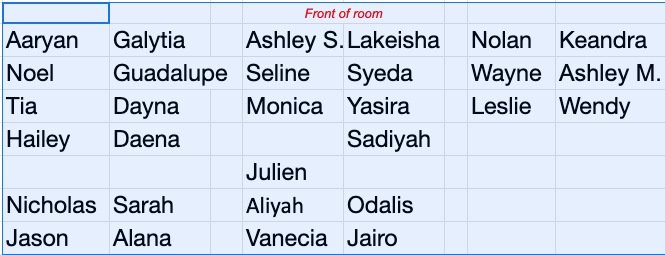
\includegraphics[width=11cm]{IB-seating-chart.png}
}

\section{4.4 Deltamath review, test corrections Tuesday 5 January}
\frame
{
  \frametitle{GQ: How do we interpret slope as rate of change?}
  \framesubtitle{CCSS: HSS.CP.A.4 Understand linear functions \hfill \alert{4.4 Tuesday 5 January}}

  \begin{block}{Do Now: Venn diagram problem}
  \begin{enumerate}
    \item Interpret the quantities in a Venn diagram
    \item Assigning quantities to a Venn diagram given a situation
    \item Interpret set notation as Venn diagram shading
  \end{enumerate}
  \end{block}
  Deltamath linear functions practice \\ \bigskip
  Spicy: Vector introduction \\ \smallskip
  Homework: Complete textbook exercises 4A-4F, Deltamath review problems
}

\section{4.5 Modeling, piecewise functions Wednesday 8 January}
\frame
{
  \frametitle{GQ: How do we model situations with multiple conditions?}
  \framesubtitle{CCSS: HSS.CP.A.4 Understand linear functions \hfill \alert{4.5 Wednesday 8 January}}

  \begin{block}{Do Now: Function and algebra review}
  \begin{enumerate}
      \item Simple function notation
      \item Calculator use with trig functions
      \item Solve literal equations algebraically 
  \end{enumerate}
  \end{block}
  Lesson: Piecewise functions pp. 165-167 \\ \smallskip
  Homework: Textbook exercises 4G p. 167
}

\end{document}
